\section{Data and descriptive characteristics}\label{sec:data}
\subsection{Sources, sample and the information clock}
Our textual inputs are public Q\&A records from the Shenzhen Stock Exchange's Easy Interaction platform and the Shanghai Stock Exchange's E-Interaction platform, obtained through CNRDS. The source supplies matched questions and replies. Stock returns, prices, financial characteristics, trading variables and listing dates come from CSMAR. We preserve the source records, production tone scores and Random Forest substantiveness scores; the integration does not retrain the classifiers or alter historical observations.

The original regression preparation retains 5,812,275 firm-day observations after its listing-age filter. ESI has complete text inputs on 1,317,473 of these observations. The original portfolio preparation has 2,553,356 complete-text observations and follows a different eligibility rule. These counts describe input pools, not final regression samples or independent questions. Table~\ref{tab:parameters} reports their separate scales. A firm day with at least one recorded inquiry is an interaction day; absence of a question is not a neutral tone. Missing tone or reply inputs are not filled with zero to manufacture an ESI observation.

Reply timing matters because an answer may arrive after the investor's question. In the historical construction, both sides of the matched dialogue are aggregated to the original company-question-date cohort. This is not separate aggregation of all questions posted today and all replies posted today. A Day~1 question and its Day~3 reply contribute to the historical Day~1 ESI, even though the completed signal was not available on Day~1. Returns attached to that question date need not follow the public release of all inputs.

The separate availability construction assigns a completed cohort to the first exchange trading day strictly after its last recorded reply; multiple cohorts arriving at the same company-availability date are combined. We denote this date by $a$ when defining its outcomes. This extension changes the clock and uses its own frozen calibration and sample. Neither construction treats an unanswered question as a completed matched dialogue.

\subsection{Construction and interpretation of ESI}\label{sec:esi_construction}
ESI combines two signed components: attention-weighted investor tone and content-weighted managerial tone. Figure~\ref{fig:esi_flow} gives the sequence before the individual steps. The aim is to represent the interaction context explicitly, not to claim that the index measures a directly observed psychological response.
\begin{figure}[H]\centering\small
\fbox{\parbox{.91\textwidth}{\centering Matched question and reply records\\Retain the original question-date cohort; distinguish later public availability}}
\par\smallskip$\Downarrow$\par\smallskip
\fbox{\parbox{.91\textwidth}{\centering Score and aggregate both tones; measure question volume and reply substantiveness}}
\par\smallskip$\Downarrow$\par\smallskip
\fbox{\parbox{.91\textwidth}{\centering Investor component: $I(1+\lambda A)$\\Managerial component: $Z^M Sub K(I)$, with original asymmetric protection}}
\par\smallskip$\Downarrow$\par\smallskip
\fbox{\parbox{.91\textwidth}{\centering Combine using frozen full-pool text scales\\Evaluate historical O2C outcomes; report availability C2C evidence separately}}
\caption{From Matched Dialogue to the Historical ESI}\label{fig:esi_flow}
\end{figure}
Separate sentiment classifiers produce negative, neutral and positive probabilities for inquiries and replies. Tone is the positive probability minus the negative probability, ranging from $-1$ to $1$. We average the respective scores within the matched firm-date cohort. Contextual scoring recognizes that financial expressions can differ from general language \citep{loughran2011}; this motivation does not establish the accuracy of the undocumented production sentiment models.

Reply substantiveness, $Sub_{i,t}$, is one minus the Random Forest probability of an evasive reply. Its inputs include lengths, Q\&A similarity, numerical and date indicators, and generic-disclosure phrases. The existing label file provides 1,999 usable substantiveness labels but lacks sufficient annotation metadata to establish independent ground truth. Appendix~\ref{app:nlp_methodology} reports a common-holdout comparison with Chinese BERT and a local instruction model. The production scores remain unchanged.

Let $I_{i,t}$ and $M_{i,t}$ denote the two mean tones, and $N_{i,t}$ the number of questions. Define
\begin{align}
A_{i,t}&=\frac{\log(1+N_{i,t})}{\max_{j,s}\log(1+N_{j,s})}, & Z^M_{i,t}&=\frac{M_{i,t}-\bar M}{\sigma_M},\\
\theta&=Q_I(0.30), & \sigma_K&=0.8\sigma_I,\\
K(I_{i,t})&=\exp\!\left[-\frac{(I_{i,t}-\theta)^2}{2\sigma_K^2}\right], & G_{i,t}&=Z^M_{i,t}Sub_{i,t}K(I_{i,t}).
\end{align}
The attention multiplier preserves investor tone's sign and lies between 1 and 1.5 when $\lambda=0.5$. Attention and tone describe distinct aspects of expressed beliefs \citep{barber2008,da2011,cookson2024}. Reply specificity moderates the contribution of managerial language, consistent with examining verifiable detail rather than optimism alone \citep{hutton2003,hollander2010}. The state weight is largest at the 30th percentile of investor tone and falls with distance. This is a modeling choice motivated by the possibility that initial affect changes how advice is processed \citep{gino2012,loewenstein2001risk}; those studies do not identify our numerical anchor or bandwidth.

The original code contains an asymmetric protection, which must also appear in the written formula:
\begin{equation}
\widetilde G_{i,t}=\begin{cases}0,& I_{i,t}>0\ \text{and}\ G_{i,t}<0,\\G_{i,t},&\text{otherwise},\end{cases}
\quad ESI_{i,t}=I_{i,t}(1+0.5A_{i,t})+5\widetilde G_{i,t}.\label{eq:esi}
\end{equation}
Below-average managerial tone therefore does not subtract from a positive investor component in that state. This truncation is a historical specification choice, not an estimated behavioral result.

Table~\ref{tab:parameters} uses the full original 2010--2024 text pools before response-lag grouping. Regression and portfolio programs use different pools; their separate means, standard deviations, anchors and attention denominators are preserved. The constants $\lambda=0.5$, $\gamma=5$, $q=0.30$ and $b=0.8$ are inherited choices. Full-sample moments explain how they translate into weights; they do not demonstrate optimality, preregistration, or an untouched out-of-sample test. Figures~\ref{fig:parameter_distribution} and \ref{fig:weights} show the distributional scale and weighting function.
\begin{table}[H]
\centering\footnotesize
\caption{Frozen Full-Sample Text Scales}\label{tab:parameters}
\begin{threeparttable}
\renewcommand{\arraystretch}{1.12}
\begin{tabular*}{\textwidth}{@{\extracolsep{\fill}}lrr@{}}
\toprule
Quantity & Regression pool & Portfolio pool \\
\midrule
Complete text observations & 1,317,473 & 2,553,356 \\
$\bar M$ & 0.1868 & 0.1690 \\
$\sigma_M$ & 0.2796 & 0.2693 \\
$Q_I(0.30)$ & -0.1417 & -0.2169 \\
$\sigma_I$ & 0.3659 & 0.3761 \\
$0.8\sigma_I$ & 0.2928 & 0.3009 \\
$\max\log(1+N)$ & 4.8040 & 5.5134 \\
$\overline{ESI}$ & 0.4857 & 0.3609 \\
$\sigma_{ESI}$ & 2.8106 & 2.5182 \\
\bottomrule
\end{tabular*}
\begin{tablenoteblock}
The original 2010--2024 analysis pools are retained separately. Regression construction excludes the first six months after listing; portfolio preparation uses its original return and market-capitalization availability rules. These are full-sample distributional scales, not an early training window or externally estimated economic parameters. $\lambda=0.5$, $\gamma=5$, $q=0.30$, and $b=0.8$ remain fixed. No per-lag recalibration is performed. The full-period construction overlaps the evaluation period.
\end{tablenoteblock}
\end{threeparttable}
\end{table}

\begin{figure}[H]\centering
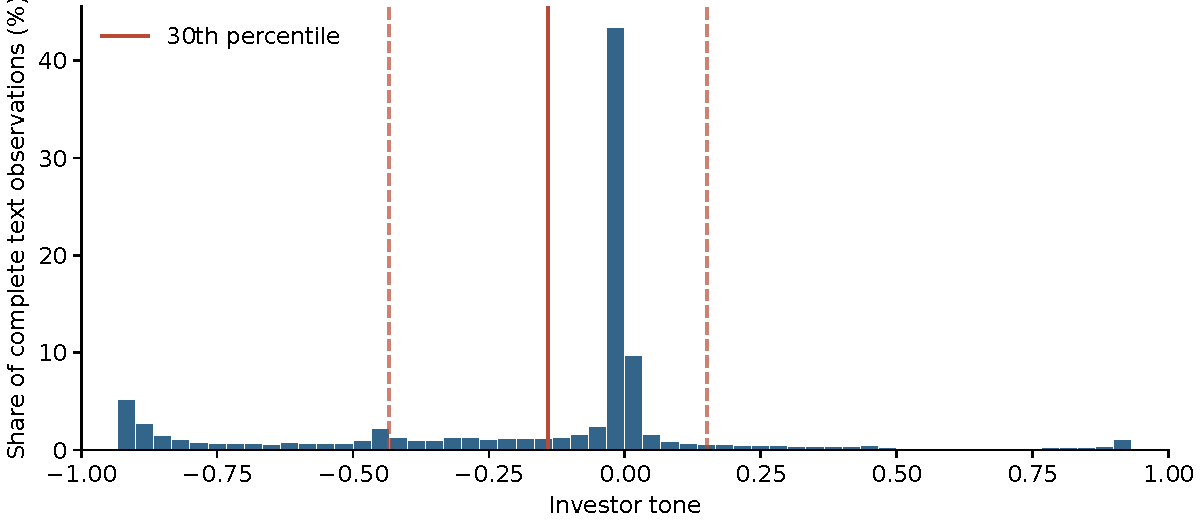
\includegraphics[width=\textwidth]{figures/investor_distribution.pdf}
\caption{Full-Regression-Pool Investor Tone and the State Anchor}\label{fig:parameter_distribution}
\footnotesize Complete text observations in the original regression pool. The solid line is the frozen 30th percentile; dashed lines are one kernel bandwidth on either side. Frequencies are descriptive and do not use returns.
\end{figure}
\begin{figure}[H]\centering
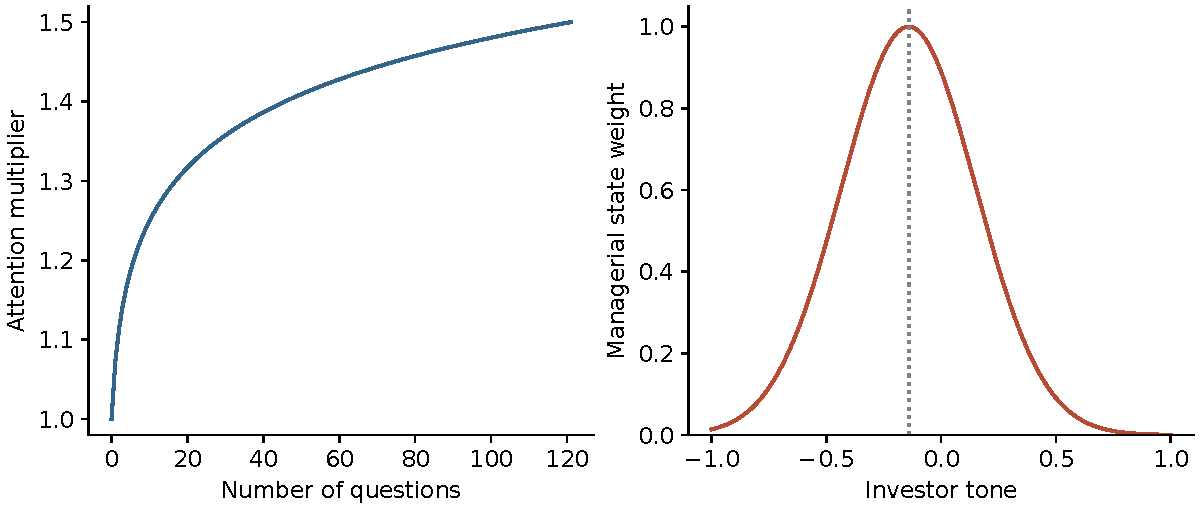
\includegraphics[width=\textwidth]{figures/esi_weights.pdf}
\caption{Historical Attention Multiplier and State Weight}\label{fig:weights}
\footnotesize Curves apply frozen regression-pool scales. The state curve is a deterministic weight, not a density estimate or fitted return response. Both pool-specific scale sets appear in Table~\ref{tab:parameters}.
\end{figure}

\subsection{Outcome and control definitions}
The historical O2C outcome is the next recorded stock day's closing price divided by its opening price minus one, less that record's risk-free rate. Excluding the overnight interval does not solve the late-reply problem. Original factor-residual outcomes use full-period firm regressions with factors indexed by the signal date. They are in-sample residuals, not rolling estimates based solely on past data.

Historical baseline regressions use eleven controls: size, book-to-market, profitability, leverage, illiquidity, turnover, prior return, trailing volatility, earlier cumulative returns, prior news tone and a news indicator. Table~\ref{tab:variables} groups them by use. News controls distinguish platform language from the prior public-information environment. Accounting inputs are inherited from the master panel; this integration does not reconstruct point-in-time revisions or publication histories. Announcement-specific controls are defined in their test rather than mixed into the baseline data description.
